
%==============================================================================
\section{ Results}
The ORB-SLAM algorithm has been successfully implemented on the hardware, adapted for ROS using C++ as the main programming language. The robot can identify key points in video data as seen in Figure \ref{fig:keypoints} and generate a map of the environment as it moves through it. The results of this mapping can be seen in Figure \ref{fig:map} below.

%% TODO: Add figure showing constructed map from ORB-SLAM

\begin{figure}[h]
    \centering
    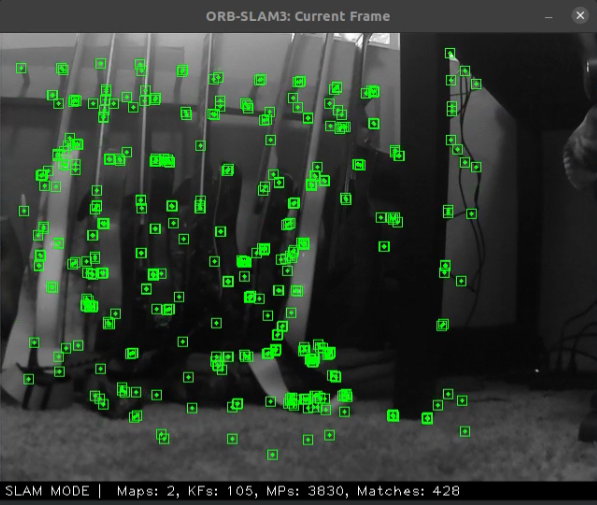
\includegraphics[scale=0.4]{figures/orb_slam3_keypoints.png}
    \caption{Example key points identified in ORB-SLAM3 from video feed}
    \label{fig:keypoints}
\end{figure}

\begin{figure}[h]
    \centering
    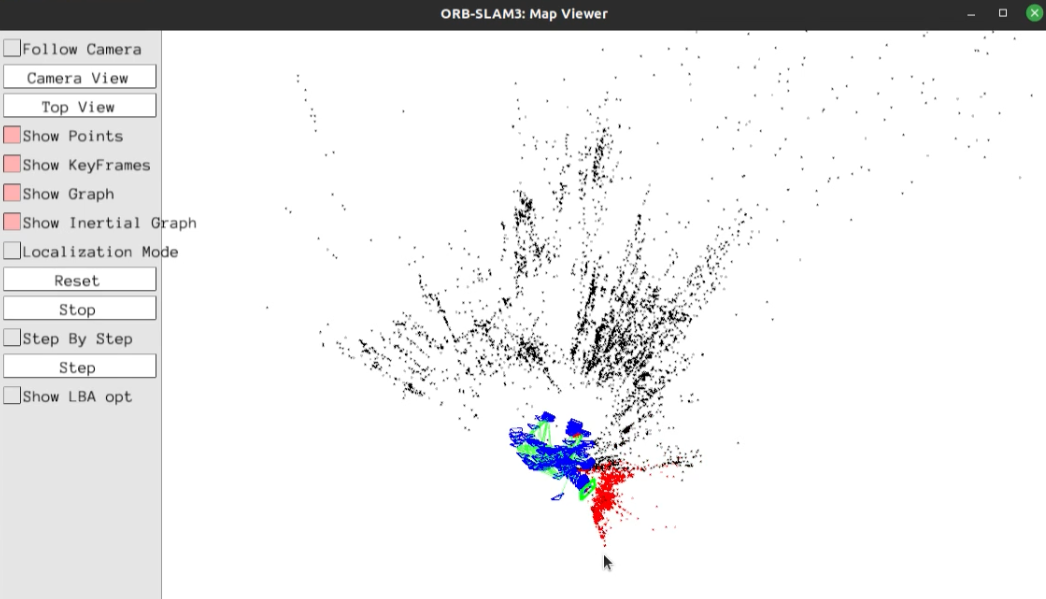
\includegraphics[scale=0.24]{figures/orb_slam3_map.png}
    \caption{ Generated Map from the Hexapod's Measurements}
    \label{fig:map}
\end{figure}

An example of the pose estimation generated from ORB-SLAM3 and the EKF can be seen in Table \ref{table:pose_data}. Truth data is obtained by measuring the true motion of the robot relative to its initial position using a tape measure. 

\begin{table}[h!]
\begin{adjustbox}{width=0.5\textwidth}
\begin{tabularx}{0.6\textwidth}{ ||c c c c c c c c ||}

    \hline
    Source & $p_x$ & $p_y$ & $p_z$ & $q_w$ & $q_x$ & $q_y$ & $q_z$ \\
    \hline \\
    Truth & -0.762 & -1.320 & 0.212 & 0.5 & 0 & 0 & -0.867 \\
    EKF & -0.6 & -0.239 & -0.822 & -0.005 & -0.007 & -0.216 & 0.976 \\
    SLAM & 0.166 & 0.030 & -0.069 & -0.011 & 0.713 & -0.153 & 0.684 \\
    \hline

\end{tabularx}
\end{adjustbox}
\caption{Pose estimation for SLAM and EKF systems}
\label{table:pose_data}
\end{table}
